% ===== CHAPTER 6: RESULTS AND ANALYSIS =====

\chapter{Results and Analysis}
\label{ch:results}

The evaluation criteria in Chapter~4 were written around a pilot with real students: time
to a confirmed companion, acceptance rate, fill rate. The pilot did not happen. The
development database holds seven accounts and seven activities created by the team, and
computing a median from five join requests would not mean anything. This chapter therefore
measures the system rather than its use: how fast it answers, how it behaves as load and
data grow, how much of it is tested, and how it grew over the semester. Every number here
was measured on 20 November 2026 on the machine described in Chapter~\ref{ch:testing}, with
the server, the database and the load generator on the same laptop. That leaves out the
network, and through the ngrok tunnel a phone will see tens of milliseconds more on every
request.

\section{Response Times}

Each endpoint was called 300 times in a row by a logged-in student after five warm-up calls
(60 times for login). Figure~\ref{fig:latency} shows the median and the 95th percentile.

\begin{figure}[htbp]
\centering
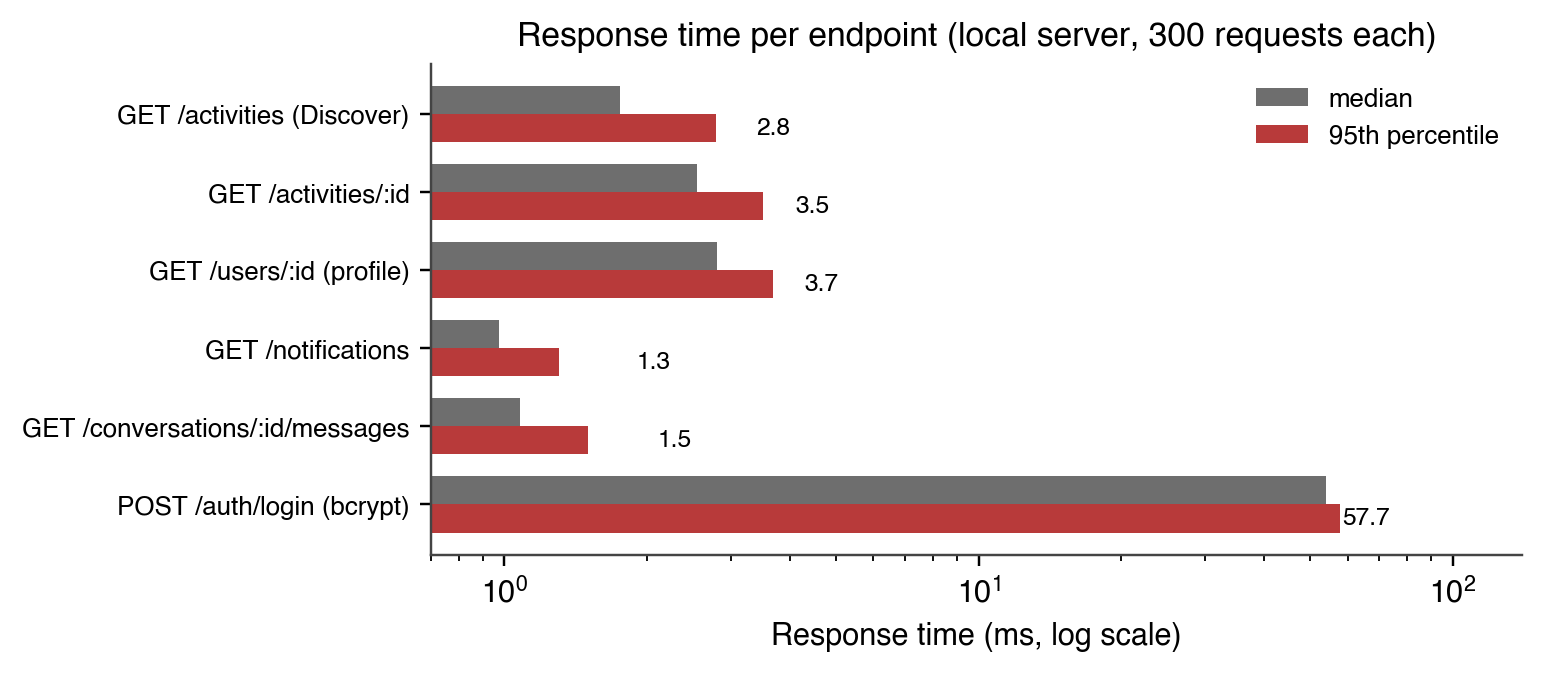
\includegraphics[width=0.92\textwidth]{figures/charts/chart-latency.png}
\caption{Server response time per endpoint}
\label{fig:latency}
\end{figure}

Every read the app makes on a normal screen answers in under 4~ms at the 95th percentile.
The profile is the slowest of them at 2.8~ms median, because it runs six queries (the user,
counts, histogram, tag counts, recent reviews and upcoming activities). Login is twenty times slower than
anything else, at 54~ms, and that is deliberate: bcrypt with ten rounds is meant to be slow,
so that a stolen password table is expensive to attack. Login happens once per device now
that sessions are saved, so its cost is paid rarely.

\section{Behaviour Under Concurrent Load}

Figure~\ref{fig:concurrency} shows Discover, the busiest screen, requested 400 times by 1, 5,
10, 25 and 50 clients at once.

\begin{figure}[htbp]
\centering
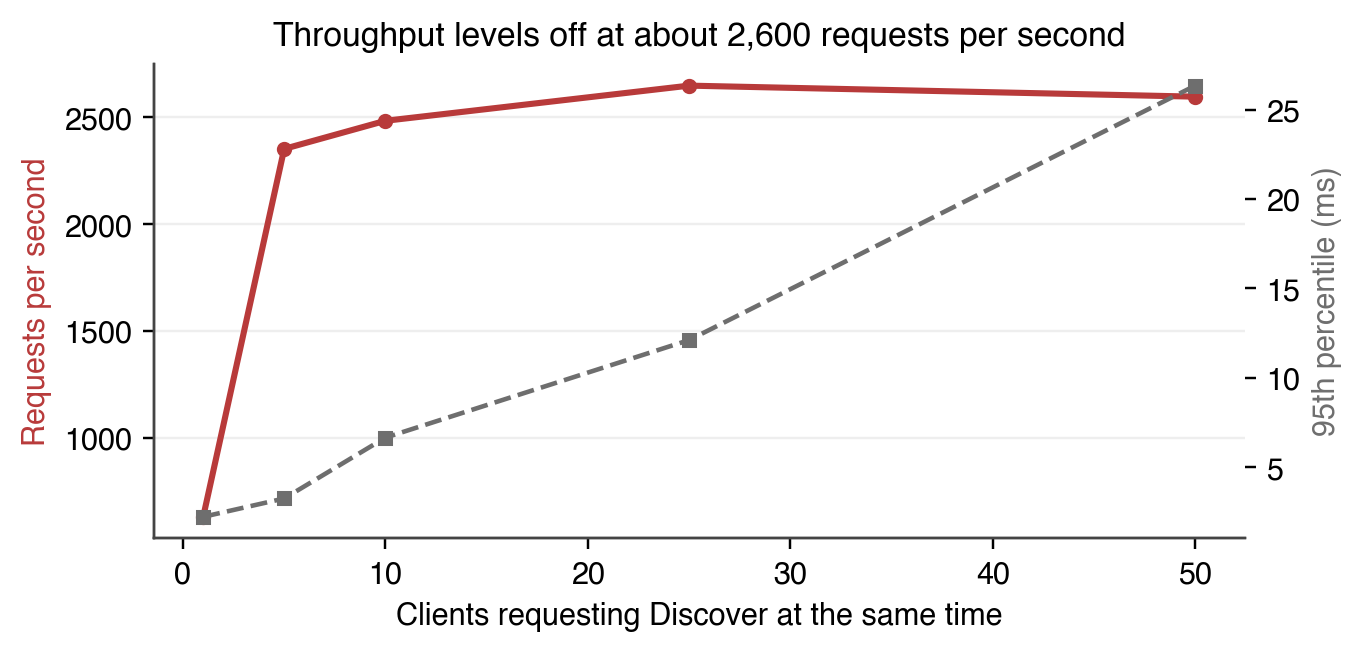
\includegraphics[width=0.92\textwidth]{figures/charts/chart-concurrency.png}
\caption{Throughput and 95th-percentile latency as concurrent clients increase}
\label{fig:concurrency}
\end{figure}

One client reaches 631 requests a second. Throughput climbs to about 2{,}350 at five clients
and then flattens at roughly 2{,}600, while the 95th percentile keeps rising, from 3.3~ms at
five clients to 26~ms at fifty. That is the shape of a single Node.js process using one core
fully: past that point extra clients only queue. For context, ten thousand
students each opening Discover once a minute would need under 170 requests a second. Capacity is not what limits this deployment; the laptop being switched off is.

\section{How Discover Scales With Data}
\label{sec:scaling}

The mid-semester report predicted that the average-rating subquery would be the first thing
to slow down. To check, activities were added to the test database in steps up to 4{,}000
and Discover was timed 30 times at each size (Figure~\ref{fig:scaling}).

\begin{figure}[htbp]
\centering
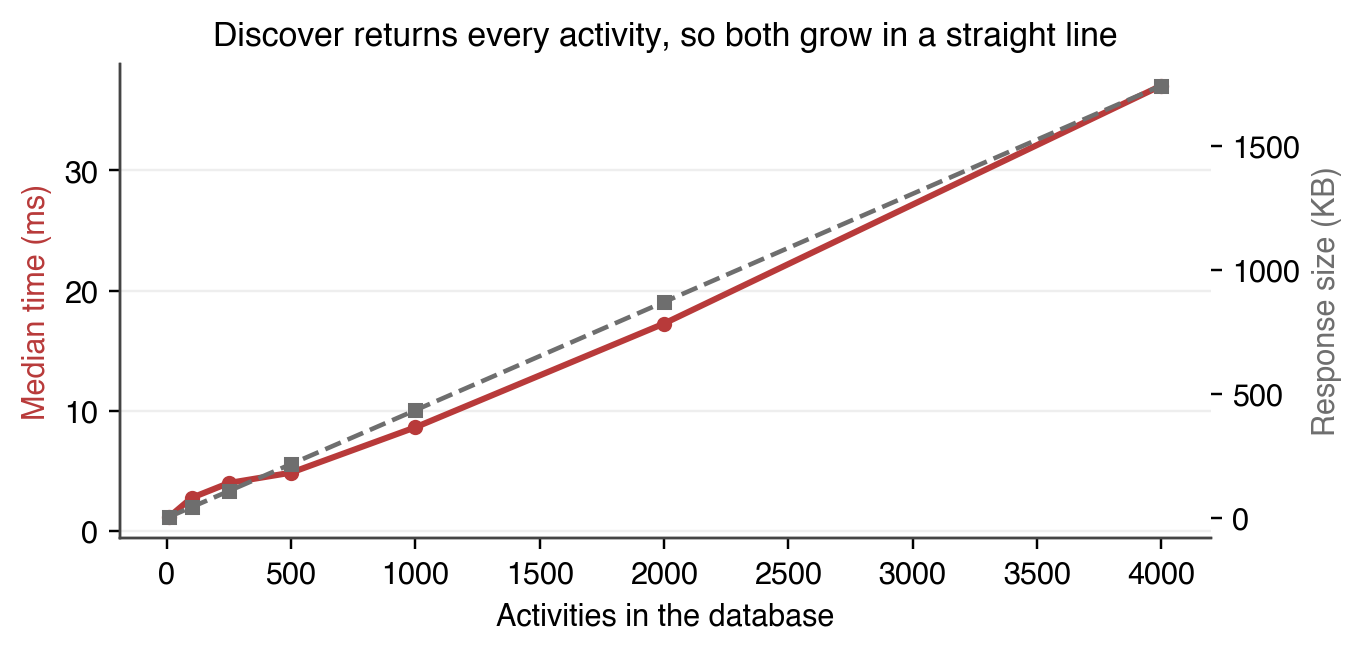
\includegraphics[width=0.92\textwidth]{figures/charts/chart-discover-scaling.png}
\caption{Discover response time and response size against the number of activities}
\label{fig:scaling}
\end{figure}

\begin{table}[htbp]
\centering
\begin{tabular}{|r|r|r|r|}
\hline
\textbf{Activities} & \textbf{Median (ms)} & \textbf{95th pct (ms)} & \textbf{Response (KB)} \\
\hline
10 & 1.2 & 2.8 & 5 \\
100 & 2.7 & 3.4 & 44 \\
500 & 4.8 & 6.1 & 217 \\
1{,}000 & 8.6 & 9.8 & 434 \\
2{,}000 & 17.3 & 19.0 & 870 \\
4{,}000 & 37.1 & 39.7 & 1{,}741 \\
\hline
\end{tabular}
\caption{Discover at increasing data sizes}
\label{tab:scaling}
\end{table}

Both lines are straight. Time grows by about 9~ms per thousand activities and the response
by about 0.43~KB per activity. The prediction was half right. The query does get slower, but
at 4{,}000 activities it still finishes in under 40~ms, which no student would notice. The
response size is the real problem: 1.7~MB sent on every visit to Discover, over mobile data,
through a tunnel with a monthly allowance. Pagination on \texttt{starts\_at}, sending the
next twenty activities as the student scrolls, would hold the response at about 9~KB
whatever the table size. That is the most useful single change left on the server.

\section{Test Coverage}

\begin{figure}[htbp]
\centering
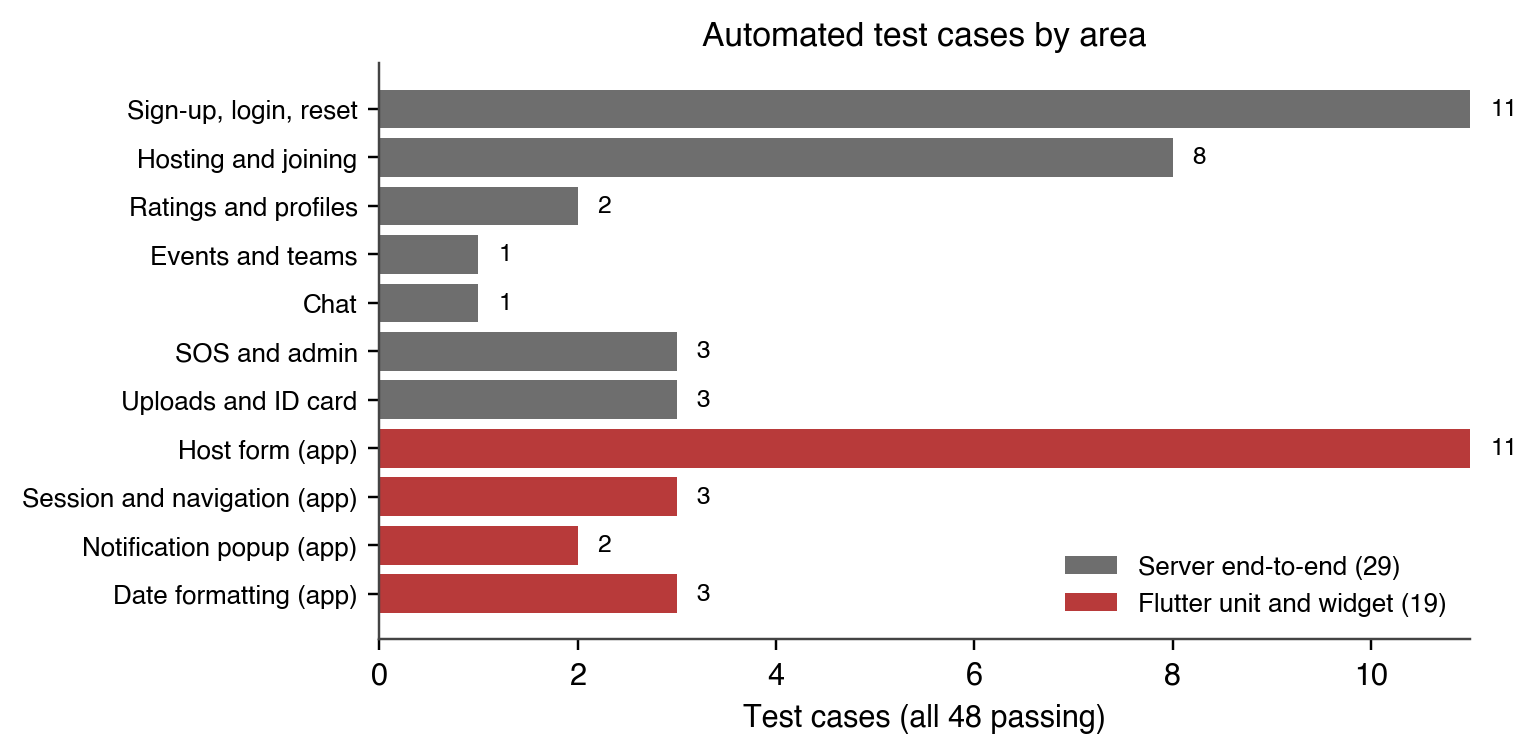
\includegraphics[width=0.92\textwidth]{figures/charts/chart-tests.png}
\caption{The 48 automated test cases by area}
\label{fig:testareas}
\end{figure}

Figure~\ref{fig:testareas} shows where the 48 tests sit. The server suite is weighted toward
sign-up and the join handshake, the two places where a mistake would let the wrong person in.
Chat, events and ratings have fewer cases each. The app tests concentrate on the host form,
which has the most input handling. What no automated test covers is the look and flow of the
screens themselves; Section~\ref{sec:screens} covered those by hand. The SOS endpoint is
tested only for refusing a student without a contact, because a passing test would send a
real text message.

\section{How the Project Grew}

\begin{figure}[htbp]
\centering
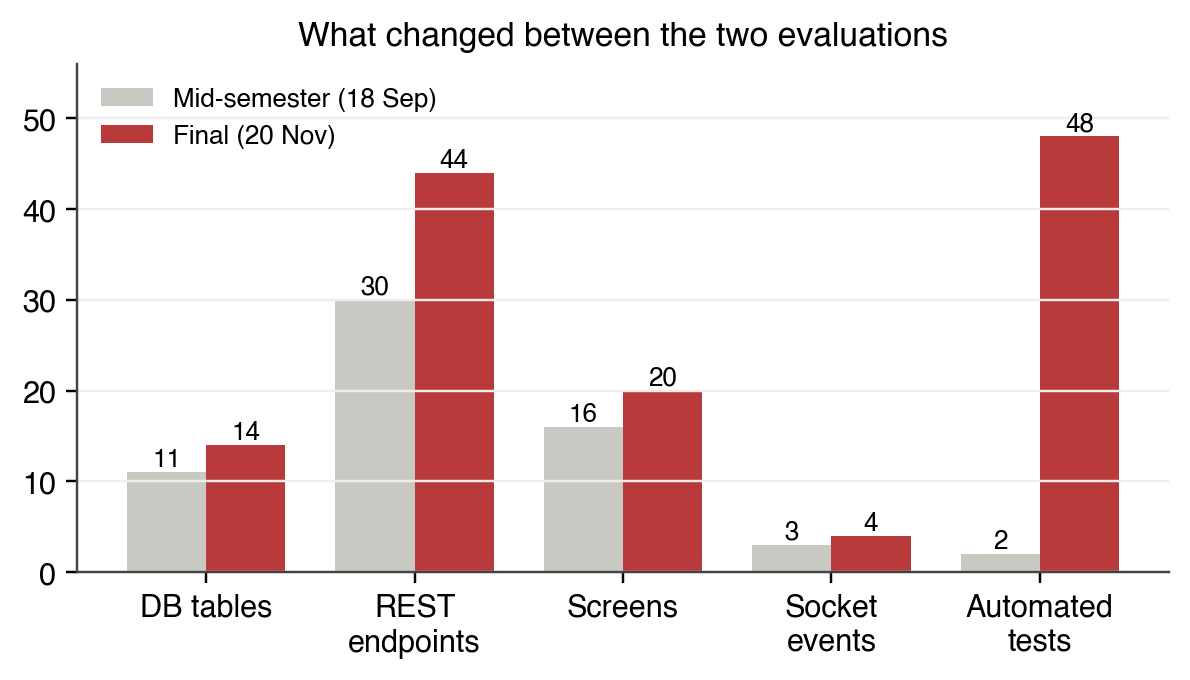
\includegraphics[width=0.92\textwidth]{figures/charts/chart-mid-vs-final.png}
\caption{The system at the two evaluations}
\label{fig:midfinal}
\end{figure}

\begin{figure}[htbp]
\centering
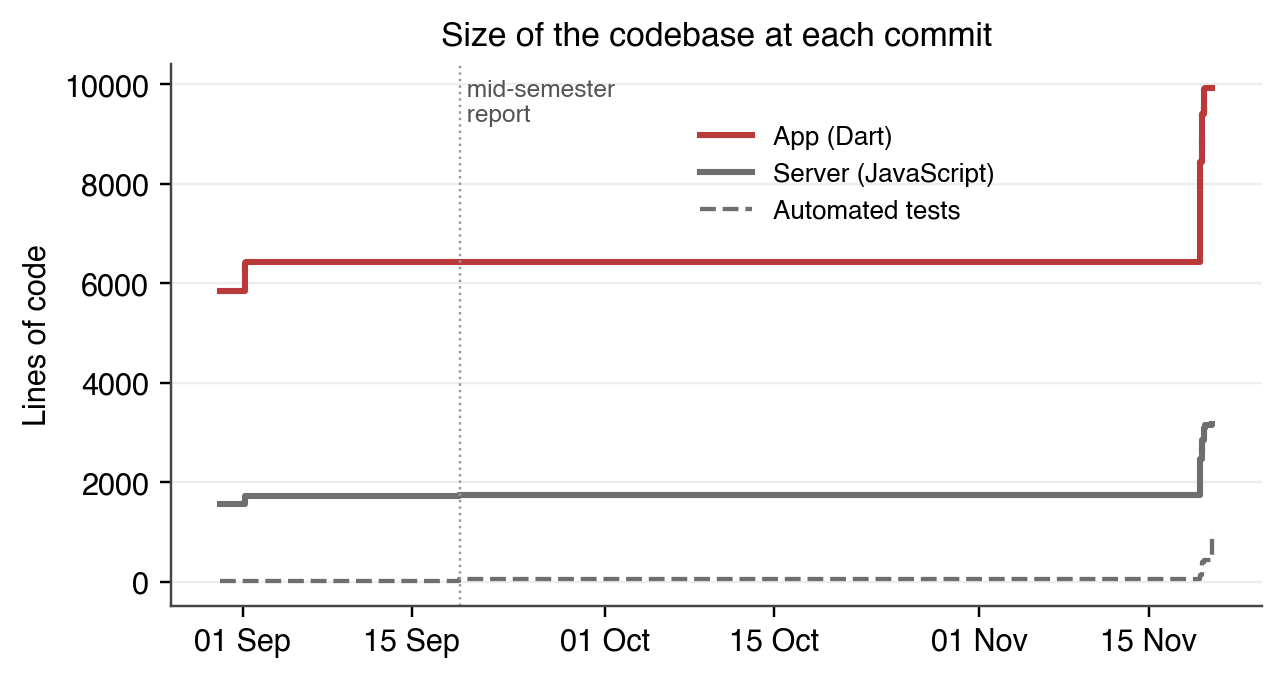
\includegraphics[width=0.92\textwidth]{figures/charts/chart-code-growth.png}
\caption{Lines of code at each commit in the local repository}
\label{fig:growth}
\end{figure}

Figure~\ref{fig:midfinal} puts the two evaluations side by side. The largest relative change
is in tests, from 2 to 48. Figure~\ref{fig:growth} counts lines at every commit. The flat
stretch between mid-semester and 19 November is an honest picture of the repository rather
than of the work: the application code was committed in bursts, and the features from
Chapter~3's Modules 8 to 14 arrived in 26 commits on 19 November. The test suite and the
report followed on 20 November. Committing more often, in smaller pieces, would have made
both the history and the journal in Chapter~\ref{ch:journal} easier to reconstruct.

\section{Summary of Findings}

\begin{itemize}
  \item The server is fast enough by a wide margin. Ordinary reads take 1 to 3~ms and one
        process handles about 2{,}600 requests a second.
  \item Discover's cost grows in a straight line with the number of activities, and the
        response size, not the query time, is what will hurt first. Pagination is the fix.
  \item 48 automated tests pass, and writing them found three defects of their own kind: a
        setup script that had never worked on a clean install, and two tests that would have
        given false confidence.
  \item Usage outcomes (time to a confirmed companion, fill rate) remain unmeasured because
        the pilot was not run.
\end{itemize}
